%  Pt1.tex
% !TeX spellcheck = en_GB
% !TeX root = ProjectRiskManagement.tex

\section{Approaches to Uncertainty and Underlying Complexity Management - 1200}

Introduction to risk and opportunity, underlying complexity. 

Challenge of traditional view of risk.

%Project life cycle introduction.
A traditional four stage view of the asset/change lifecycle is a useful starting point to consider the scope of a project.
The four stages are conceptualize, planning, execution and delivery (E\&D) and Utilization.
Effective uncertainty management requires a macro-view of the entire project context, so that corporate and operational uncertainty is captured in addition to planning uncertainty.
This leads to an elaboration of the lifecycle to incorporate 12 stages, each emphasizing a different management purpose and outcome.
Both views are shown in figure \ref{Figure:Project_Lifecycle}.

This paper is particularly concerned with the E\&D strategy shaping phase.
This is within the broader planning cqtegory, and follows the design,operation and termination strategy shaping phase.
The DOT phase aims are to ...
The E\



\begin{figure}[!h]
  \centering
    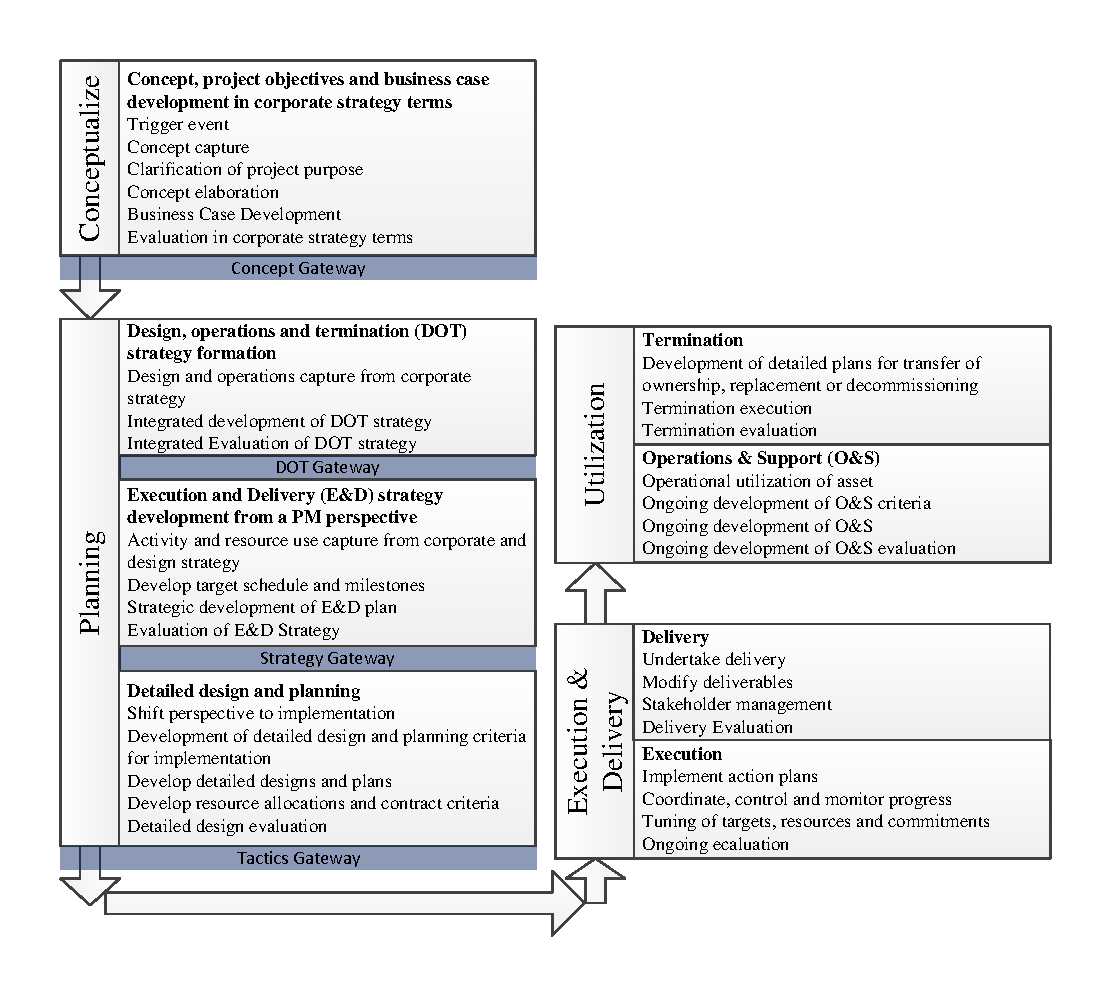
\includegraphics[width = \textwidth]{./Figures/ProjectLifecycleDetailedCurve.pdf} 
\caption{Twelve-stage asset/change lifecycle - adapted from \cite{chapman}}
\label{Figure:Project_Lifecycle}
\end{figure}

% execution and delivery strategy shaping phase of a project's life cycle
Procedures are a common way to ensure consistency and quality is maintained through a range of repeated applications.
While a good procedure is often designed to be simple, repeatable and transparent, this cannot be a uniform approach.
Some high complexity, high uncertainty projects require sophisticated, tailored procedures.
The PUMP framework supports this concept through the idea of PUMP packs, that is a set of PUMPs tailored to specific projects and project lifecycle stages.
This paper focusses on PUMPs within the context of the E\&D strategy shaping stage.


\subsection{The PUMP Process}
%Explain concisely in your own words what you believe are the key overall features of a PUMP approach to project risk management in the execution and delivery strategy shaping phase of a project’s lifecycle. Compare these features with the PMI PIMBOK approach or any other form of common practice you are familiar with if you find this helpful, but focus on the PUMP approach. Use examples to illustrate your discussion if you wish, but concentrate on concepts and principles. This will be a largely descriptive summary of your interpretation of the lectures and associated reading. It will demonstrate your grasp of the central core of the unit’s material as a whole, and should be approached with a view to demonstrating this understanding..



\subsection{Contrast with Other Risk Management Processes}
Contrast with PUMP and PMI PMBOK and others.

\subsection{The Clarity Efficient Approach}
Summarise that PUMPS offer a higher level of clarity for the project as a whole rather than 


1200words.